\documentclass[12pt]{article}
\usepackage{graphics}
\usepackage{amsmath}
\usepackage{mathtools}
\usepackage{gensymb}

\newcommand{\mydet}[1]{\ensuremath{\begin{vmatrix}#1\end{vmatrix}}}
\providecommand{\brak}[1]{\ensuremath{\left(#1\right)}}
\providecommand{\norm}[1]{\left\lVert#1\right\rVert}
\newcommand{\solution}{\noindent \textbf{Solution: }}
\newcommand{\myvec}[1]{\ensuremath{\begin{pmatrix}#1\end{pmatrix}}}
\let\vec\mathbf

\begin{document}
\begin{center}
\textbf\large{CHAPTER-7 \\ COORDINATE GEOMETRY}

\end{center}
\section*{Excercise 7.2}

Q7.Find the coordinates of point A, where AB is the diameter of a circle where the center is (2,-3) and B is the point (1,4):
\begin{enumerate}
	\item $B\brak{1,4}, C\brak{-2,3}$
\end{enumerate}
\solution
\begin{enumerate}
\item The coordinates are given as
	\begin{align}
	\vec{B} = \myvec{
		1\\
	    4\\
		},
	\vec{C} = \myvec{
	   -2\\
		3\\
		},
	\end{align}
	
In a straight line AB, whose coordinates are A(x1,y1) and B(x2,y2). The mid-point of AB is C(x,y). 
	


Let us assume the coordinate of A as (x,y). Now, as the center is the midpoint of AB, which is given in the start as (2, -3) and we have B as (1,4).
		
Hence,	
			C = $\frac{1}{2}(A+B)$
	\begin{align}
	\myvec{
	    2\\
	   -3\\
		} &= \frac{A+B}{2} \\
		\myvec{
	    2\\
	   -3\\
		} &= \frac{1}{2}\brak{\myvec{x\\y\\}+\myvec{1\\4\\}} \\
		\myvec{
	    2\\
	   -3\\
		} &= \frac{1}{2}\myvec{x+1\\y+4\\}\\
		\myvec{
	    2\\
	   -3\\
		} &= \myvec{(x+1)/2\\(y+4)/2\\}	
	\end{align}       
	 From equation (5) we need to find the values of x and y which are the coordinates of A. Thus,
    \begin{align}
	\begin{split}	                     
	{(x+1)/2} = 2\\
	\implies  
	\brak{(x+1)}& = 4 \\
	\implies 
	\brak{x}& = (3)\\
    \end{split}
    \end{align}
    Similarly,
    \begin{align}
    \begin{split}
    {(y+4)/2} = -3\\
    \implies
    \brak{(y+4)}& = -6 \\
    \implies
    \brak {y}& = (-10)\\
    \end{split}
    \end{align}
    Hence, therefore value of x and y for given point B(1,4) and center C(-2,3) is 3 and -10 respectively. So the coordinates of A is given by 
    A(x,y) = A(3,-10).	
\hspace{3mm}
\begin{figure}[!h]
\begin{center}	
	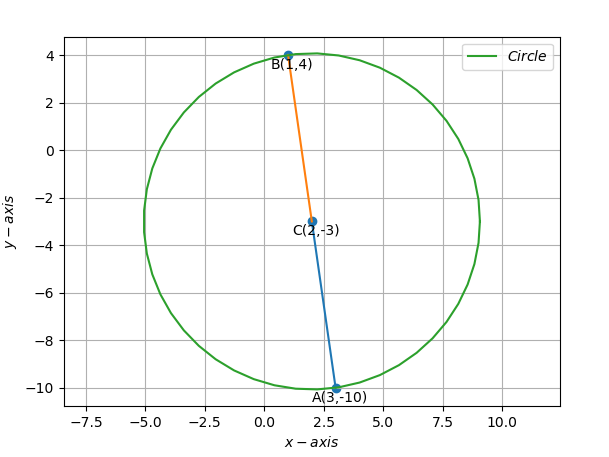
\includegraphics[width=6in]{Vector1.png}
\end{center}
\caption{Circle for the given coordinates}
\label{fig:Fig}
\end{figure}
\end{enumerate}
\end{document}
	
